\documentclass[11pt,oneside]{article}

\usepackage[a4paper,margin=25mm,headheight=15pt]{geometry}
\usepackage[T1]{fontenc}
\usepackage[utf8]{inputenc}
\IfFileExists{libertinus.sty}{\usepackage{libertinus}}{\usepackage{lmodern}}
\usepackage{microtype}
\usepackage{amsmath,amssymb,amsthm,mathtools,mathrsfs,bm}
\usepackage{booktabs,longtable,tabularx,array,multirow}
\usepackage{graphicx}
\usepackage{xcolor}
\usepackage{enumitem}
\usepackage{fancyhdr}
\usepackage{titlesec}
\usepackage{xurl}
\usepackage{listings}
\usepackage{siunitx}
\usepackage{hyperref}
\usepackage[nameinlink,noabbrev]{cleveref}

\definecolor{linkblue}{RGB}{25,75,135}
\definecolor{deepgreen}{RGB}{25,105,74}
\definecolor{deepred}{RGB}{145,43,43}
\definecolor{shadegray}{RGB}{246,247,249}
\definecolor{rulegray}{RGB}{195,201,208}
\hypersetup{
  colorlinks=true,
  linkcolor=linkblue,
  citecolor=deepgreen,
  urlcolor=linkblue,
  pdftitle={Dyadic-Comb Interpolation of the Fabius and Rvachev Functions},
  pdfauthor={OpenAI GPT-5.6 Pro},
  pdfsubject={Runge instability, endpoint-flat Hermite constraints, exact cardinal obstructions, and numerical experiments},
  pdfkeywords={Fabius function, Rvachev up-function, Lagrange interpolation, Hermite interpolation, Runge phenomenon, dyadic comb, Lebesgue constant, Thue-Morse, q-binomial, Lambert W}
}

\pagestyle{fancy}
\fancyhf{}
\fancyhead[L]{\small Dyadic-comb interpolation}
\fancyhead[R]{\small\nouppercase{\leftmark}}
\fancyfoot[C]{\thepage}
\renewcommand{\headrulewidth}{0.4pt}

\titleformat{\section}{\Large\bfseries\color{linkblue}}{\thesection}{0.72em}{}
\titleformat{\subsection}{\large\bfseries\color{linkblue}}{\thesubsection}{0.65em}{}
\titleformat{\subsubsection}{\normalsize\bfseries\color{deepgreen}}{\thesubsubsection}{0.58em}{}
\setcounter{tocdepth}{2}
\setcounter{secnumdepth}{3}
\numberwithin{equation}{section}
\allowdisplaybreaks[3]
\setlength{\emergencystretch}{3em}
\setlist[itemize]{leftmargin=2em,itemsep=0.25em,topsep=0.45em}
\setlist[enumerate]{leftmargin=2.3em,itemsep=0.25em,topsep=0.45em}
\sisetup{scientific-notation=true,round-mode=figures,round-precision=5}

\newtheorem{theorem}{Theorem}[section]
\newtheorem{proposition}[theorem]{Proposition}
\newtheorem{lemma}[theorem]{Lemma}
\newtheorem{corollary}[theorem]{Corollary}
\newtheorem{conjecture}[theorem]{Conjecture}
\newtheorem{problem}[theorem]{Open problem}
\theoremstyle{definition}
\newtheorem{definition}[theorem]{Definition}
\newtheorem{algorithm}[theorem]{Algorithm}
\newtheorem{example}[theorem]{Example}
\theoremstyle{remark}
\newtheorem{remark}[theorem]{Remark}
\newtheorem{warning}[theorem]{Warning}

\newcommand{\R}{\mathbb R}
\newcommand{\C}{\mathbb C}
\newcommand{\Q}{\mathbb Q}
\newcommand{\N}{\mathbb N}
\newcommand{\Z}{\mathbb Z}
\newcommand{\F}{F}
\newcommand{\upf}{\operatorname{up}}
\newcommand{\e}{\mathrm e}
\newcommand{\ii}{\mathrm i}
\newcommand{\dd}{\,\mathrm d}
\newcommand{\bigO}{\mathcal O}
\newcommand{\smallo}{o}
\newcommand{\supp}{\operatorname{supp}}
\newcommand{\Leb}{\Lambda}
\newcommand{\Wgt}{W}
\newcommand{\Hbin}{H}
\newcommand{\repo}{\textsc{ProveIt}}
\newcommand{\statusproved}{\textcolor{deepgreen}{\textbf{proved here}}}
\newcommand{\statusnumeric}{\textcolor{linkblue}{\textbf{numerically verified}}}
\newcommand{\statusopen}{\textcolor{deepred}{\textbf{conjectural/open}}}
\newcommand{\fall}[2]{#1^{\underline{#2}}}

\newenvironment{resultbox}[1]{%
  \par\medskip\noindent\begin{center}\begin{minipage}{0.94\textwidth}%
  \color{deepgreen}\hrule\vspace{0.65em}%
  \color{black}\textbf{\color{deepgreen}#1.}\ }{%
  \par\vspace{0.65em}\color{deepgreen}\hrule
  \end{minipage}\end{center}\medskip}

\newenvironment{statusbox}[1]{%
  \par\medskip\noindent\begin{center}\begin{minipage}{0.94\textwidth}%
  \color{linkblue}\hrule\vspace{0.65em}%
  \color{black}\textbf{\color{linkblue}#1.}\ }{%
  \par\vspace{0.65em}\color{linkblue}\hrule
  \end{minipage}\end{center}\medskip}

\lstdefinestyle{python}{
  language=Python,
  basicstyle=\ttfamily\small,
  backgroundcolor=\color{shadegray},
  frame=single,
  rulecolor=\color{rulegray},
  columns=fullflexible,
  breaklines=true,
  keepspaces=true,
  showstringspaces=false,
  keywordstyle=\color{linkblue}\bfseries,
  commentstyle=\color{deepgreen},
  stringstyle=\color{deepred}
}

\title{\bfseries Dyadic-Comb Interpolation of the Fabius and Rvachev Functions\\[0.3em]
\large Runge instability, endpoint-flat Hermite constraints, exact cardinal obstructions,\\
and a logarithmically thin stabilization window}
\author{OpenAI GPT-5.6 Pro\\[0.3em]
\small Research report prepared from the recursive \texttt{*.tex} corpus under\\[-0.1em]
\small\path{Analysis/FabiusFunction/docs}}
\date{28 August 2026\\
\small Repository main snapshot \texttt{3c7f2912a47433264f52ad530cc75adbaa83b764}}

\begin{document}
\maketitle

\begin{abstract}
Let $N=2^n$ and interpolate the Fabius function $F$ at the complete dyadic comb
$x_j=j/N$, $0\le j\le N$.  Despite $F\in C^\infty$ and despite its flatness at both
endpoints, the ordinary global Lagrange interpolant exhibits an unmistakable Runge
transition: on an exact dyadic test grid its maximum error is about
$3.80\times10^{-3}$ at $N=16$, $4.99$ at $N=32$, $3.59\times10^7$ at $N=64$, and
$3.84\times10^{22}$ at $N=128$.  The oscillation is concentrated in narrow boundary
layers.  Exact rational computation of the endpoint derivative of the interpolant gives
still stronger evidence: $\log_2|P_N'(0)|$ is $949.99$ at $N=1024$ and $8070.57$ at
$N=8192$, although $F'(0)=0$.

We then impose the natural endpoint jets
$P^{(r)}(0)=P^{(r)}(1)=0$ for $1\le r\le m$, while preserving every dyadic value.
The resulting confluent interpolation problem has an exact factorization
\[
 P_{N,m}(x)=I_x(m+1,m+1)+[x(1-x)]^{m+1}Q_{N,m}(x),
\]
where $Q_{N,m}$ is an ordinary interpolant on the interior comb.  This converts the
large confluent system into a rational barycentric problem and applies verbatim to the
centered Rvachev bump, with the beta-polynomial bridge omitted.  At $N=64$ the Fabius
error falls from $3.59\times10^7$ to $1.78\times10^{-6}$ near $m=14$, but rises again
to $1.13\times10^3$ by $m=24$.  Matching first derivatives at \emph{every} node is much
worse: its error is already $1.54\times10^7$ at $N=32$.

The reversal is explained by two exact cardinal modes.  One mode carries boundary
perturbations toward the center and decreases with $m$; the other carries near-boundary
perturbations toward a point just off the center and grows with $m$.  Balancing them gives
an explicit predicted order
\[
 m_{\rm bal}+1=\frac{\log(A_N/B_N)}{\log(b_N/a_N)}
       \sim \frac{N\log2}{\log N},
\]
which predicts the experimentally optimal jet order surprisingly well.  The admissible
window has width only $\asymp N/(\log N)^2$.  We prove, however, that no choice of
$m=m_N$ stabilizes global equispaced interpolation in the worst-case sense: the weighted
Lebesgue constant remains at least $\exp(cN)$ for all sufficiently large dyadic $N$.
Thus endpoint flatness gives spectacular, structure-dependent finite-resolution
cancellation, not a cure for the equispaced polynomial instability.

The report includes exact formulas, proofs, high-precision experiments, unproved
conjectures on the Fabius-specific boundary layer and endpoint derivative defect, stable
replacement algorithms, and a Lean formalization program.  The accompanying Python source
reproduces every numerical table and figure using exact rational dyadic samples.
\end{abstract}

\tableofcontents
\clearpage

\section{Provenance, audit boundary, and status discipline}
\label{sec:provenance}

\subsection{Repository audit}

The source boundary is the recursive documentation tree
\path{Analysis/FabiusFunction/docs} in the public \repo{} repository.  GitHub's indexed
snapshot at commit
\texttt{fa53516af8cbe7d792a97b25378b228b96e37cf9} contained $84$ TeX paths under this
tree.  The three commits between that index and the current main snapshot
\texttt{3c7f2912a47433264f52ad530cc75adbaa83b764} changed no interpolation source and no
TeX path relevant to the present question; the only modified TeX file records a new
prefix-kernel counting formalization.

The audit distinguished living syntheses from frozen or duplicated historical revisions.
The following were treated as the primary project state:
\begin{itemize}
\item \path{Fabius_Function_and_Rvachev_Up/Fabius_Function_and_Rvachev_Up.tex};
\item \path{FabiusFunction_Mathematical_Glossary/FabiusFunction_Mathematical_Glossary.tex};
\item \path{fabius_lean_walkthrough/fabius_lean_walkthrough.tex};
\item \path{non-formalized-research-frontiers/non-formalized-research-frontiers.tex};
\item the consolidated frontier drafts under
      \path{non-formalized-research-frontiers/drafts};
\item the archived dyadic, $q$-series, inverse-function, asymptotic, and representation
      studies, together with the transcribed source papers under \path{papers}.
\end{itemize}
Every TeX path was inventoried.  Living expositions and every section found by the terms
\emph{Lagrange}, \emph{interpolation}, \emph{dyadic}, \emph{Newton}, \emph{Hermite},
\emph{Runge}, \emph{Richardson}, and \emph{sampling} were read in detail; archived
revisions were compared through their provenance and coverage ledgers rather than counted
as independent prior results.

\subsection{Novelty boundary}

The audited corpus already contains exact dyadic arithmetic, Gaussian $q$-binomial
interpolation on \emph{geometric} nodes, finite-difference and Newton-basis formulas,
Richardson transforms, all-orders endpoint asymptotics, Lambert-$W$ coordinates, and
Thue--Morse/Prouhet cancellation.  It does \emph{not} contain an analysis of global
polynomial interpolation on the complete \emph{uniform dyadic comb}, a Runge study for
$F$ or $\upf$, endpoint-flat confluent interpolation, the two cardinal obstructions derived
below, or the universal instability theorem of \cref{thm:universal-instability}.  A search
for ``Runge'' in the repository returned no result.

\begin{statusbox}{Claim labels}
A statement marked \statusproved{} has a proof in this report.  A numerical statement
marked \statusnumeric{} is reproduced by the accompanying exact-rational/high-precision
program.  Statements marked \statusopen{} are deliberately presented as conjectures or
research problems, even when the numerical evidence is strong.
\end{statusbox}

\section{Executive findings}
\label{sec:executive}

The answer to ``does Runge's phenomenon occur?'' is yes in every operational sense tested.
Ordinary global interpolation is initially accurate, then acquires enormous alternating
boundary spikes.  The evidence is stronger than a floating-point plot: all function values
are exact rationals; increasing arithmetic precision does not change the result; and an
exact rational endpoint derivative grows almost like $2^N$.

The answer to ``can higher derivatives suppress it?'' has three layers.
\begin{enumerate}
\item Fixing the \emph{natural flat endpoint derivatives} can suppress the actual Fabius or
      Rvachev error by many orders of magnitude at a given $N$.
\item The jet order must be tuned.  Too few constraints leave the ordinary boundary mode;
      too many create a reverse mode from the center toward the boundary.  The useful order
      is $m\asymp N/\log N$, in a window of width only $\asymp N/(\log N)^2$.
\item No tuning stabilizes arbitrary value data.  The global operator remains exponentially
      ill-conditioned.  Matching derivatives at every node is particularly destructive.
\end{enumerate}

\begin{resultbox}{Main frontier result}
For every sufficiently large dyadic $N$ and every endpoint jet order $m\ge0$, the weighted
Lebesgue constant of the endpoint-flat value interpolation operator satisfies
\[
  \Leb_{N,m}\ge C\e^{cN}
\]
with absolute constants $c,C>0$.  Thus a growing endpoint jet can move and temporarily
cancel the Runge instability for the special Fabius/Rvachev data, but cannot remove the
underlying equispaced polynomial instability.
\end{resultbox}

\section{Fabius and Rvachev prerequisites}
\label{sec:preliminaries}

\subsection{Normalization}

We work on $[0,1]$ with the standard Fabius function $F$, normalized by
\begin{equation}
 F(0)=0,\qquad F(1)=1,\qquad F(1-x)=1-F(x),
 \label{eq:fabius-symmetry}
\end{equation}
and satisfying
\begin{equation}
 F'(x)=2F(2x),\qquad 0\le x\le \tfrac12.
 \label{eq:fabius-differential}
\end{equation}
The centered Rvachev bump is
\begin{equation}
 u(x):=\upf(2x-1)=F(1-|2x-1|)=F\bigl(2\min(x,1-x)\bigr),
 \qquad 0\le x\le1.
 \label{eq:up-fabius}
\end{equation}
Then $F'(x)=2u(x)$ on $[0,1]$.  Both $F$ and $u$ are $C^\infty$ and flat at the relevant
boundary points:
\begin{equation}
 F^{(r)}(0)=F^{(r)}(1)=0\quad(r\ge1),
 \qquad
 u^{(r)}(0)=u^{(r)}(1)=0\quad(r\ge0).
 \label{eq:flatness}
\end{equation}

The same differential self-similarity that creates flatness also produces enormous global
derivative norms.  The audited project proves the estimate
\begin{equation}
 \lVert F^{(r)}\rVert_\infty\le 2^{r(r+1)/2}.
 \label{eq:derivative-growth}
\end{equation}
This tension---endpoint flatness versus superexponential derivative growth---is central to
why elementary interpolation remainder estimates are misleading here.

\subsection{Exact dyadic values}

Write
\begin{equation}
 V_n:=F(2^{-n}),\qquad V_0=1.
\end{equation}
The exact inverse-power recurrence used in the experiments is
\begin{equation}
 V_n=\frac{2^{-n(n-1)/2}}{2^n-1}
       \sum_{k=0}^{n-1}\frac{2^{k(k-1)/2}V_k}{(n-k+1)!}.
 \label{eq:V-recurrence}
\end{equation}
For $0<a<2^e$, set
\begin{equation}
 b=\lfloor\log_2a\rfloor,\qquad r=e-b,\qquad q=a-2^b,
 \qquad y=\frac{q}{2^e},
\end{equation}
and define
\begin{equation}
 T_r(y)=\sum_{j=0}^{r}
        \frac{2^{j(j+1)/2}}{j!}V_{r-j}y^j.
 \label{eq:T-block}
\end{equation}
The bit recursion is
\begin{equation}
 F\!\left(\frac{a}{2^e}\right)
   =T_r\!\left(\frac{q}{2^e}\right)
    -F\!\left(\frac{q}{2^e}\right).
 \label{eq:bit-recursion}
\end{equation}
Equations \eqref{eq:V-recurrence}--\eqref{eq:bit-recursion} evaluate every sample in exact
rational arithmetic.  No numerical ODE, truncated Fourier product, or spline surrogate is
used in the reported error scans.

\section{Ordinary Lagrange interpolation on the dyadic comb}
\label{sec:ordinary}

Let $N=2^n$, $x_j=j/N$, and let $L_Nf$ denote the unique polynomial of degree at most $N$
with
\begin{equation}
 (L_Nf)(x_j)=f(x_j),\qquad 0\le j\le N.
\end{equation}

\subsection{Barycentric and Newton forms}

For equispaced nodes the barycentric weights are proportional to
$(-1)^j\binom Nj$.  Hence
\begin{equation}
 (L_Nf)(x)=
 \frac{\displaystyle\sum_{j=0}^{N}
      \frac{(-1)^j\binom Nj}{x-j/N}f(j/N)}
      {\displaystyle\sum_{j=0}^{N}
      \frac{(-1)^j\binom Nj}{x-j/N}},
 \label{eq:barycentric-ordinary}
\end{equation}
away from the nodes, with the usual exact-node convention.  In forward-difference form,
\begin{equation}
 (L_Nf)(x)=\sum_{k=0}^{N}\Delta_{1/N}^{k}f(0)\binom{Nx}{k}.
 \label{eq:newton-ordinary}
\end{equation}
The appearance of the ordinary binomial coefficients in
\eqref{eq:barycentric-ordinary}, and the half-base $q$-binomial arithmetic in the dyadic
samples themselves, already hints at a mixed $q=1$/$q=1/2$ transform; we return to this in
\cref{sec:q-connections}.

\subsection{Symmetry and an exact degree drop}

\begin{proposition}[Symmetry of the Fabius interpolant]
\label{prop:symmetry}
For even $N$,
\begin{equation}
 (L_NF)(1-x)=1-(L_NF)(x).
 \label{eq:interpolant-symmetry}
\end{equation}
Consequently $L_NF$ has degree at most $N-1$.
\end{proposition}

\begin{proof}
The polynomial $1-(L_NF)(1-x)$ takes the value $F(j/N)$ at every node by
\eqref{eq:fabius-symmetry}; uniqueness gives \eqref{eq:interpolant-symmetry}.  Centering at
$x=1/2$ shows that $(L_NF)(1/2+y)-1/2$ is odd in $y$.  Its a priori degree bound $N$ is
even, so the leading coefficient vanishes.
\end{proof}

Equivalently, the top forward difference satisfies
\begin{equation}
 \Delta_{1/N}^{N}F(0)=0
 \qquad (N\ \text{even}).
 \label{eq:top-difference-zero}
\end{equation}
This cancellation is exact but does not protect the lower coefficients from exponential
growth.

\subsection{Endpoint derivatives and signed Stirling transforms}

Let $s(k,r)$ denote the signed Stirling number of the first kind,
$\fall{z}{k}=\sum_{r=0}^{k}s(k,r)z^r$.  Differentiating
\eqref{eq:newton-ordinary} gives
\begin{equation}
 (L_Nf)^{(r)}(0)
 =r!N^r\sum_{k=r}^{N}\frac{s(k,r)}{k!}\Delta_{1/N}^{k}f(0).
 \label{eq:stirling-endpoint}
\end{equation}
For $f=F$ and even $N$, the $k=N$ term vanishes by
\eqref{eq:top-difference-zero}.  In particular,
\begin{equation}
 (L_NF)'(0)=
 N\sum_{j=1}^{N}(-1)^{j+1}\binom Nj\frac{F(j/N)}{j}.
 \label{eq:endpoint-derivative}
\end{equation}
Every term of \eqref{eq:endpoint-derivative} is rational, so the derivative defect can be
computed exactly before taking a logarithm.

\subsection{Observed Runge transition}

The maximum errors below were sampled on the complete grid of mesh $2^{-12}$, except the
$N=128$ pilot scan, which used mesh $2^{-11}$.  Every target value was exact.

\begin{table}[htbp]
\centering
\caption{Ordinary global Lagrange interpolation of $F$ on the complete dyadic comb.}
\label{tab:ordinary-errors}
\begin{tabular}{rrrr}
\toprule
$N$ & degree bound & sampled $\lVert L_NF-F\rVert_\infty$ & location of largest error \\
\midrule
4   & 4   & $3.9966199\times10^{-2}$ & boundary layer \\
8   & 8   & $9.4867660\times10^{-3}$ & boundary layer \\
16  & 16  & $3.7966209\times10^{-3}$ & boundary layer \\
32  & 32  & $4.9893489$               & $x\approx0.00708$ \\
64  & 64  & $3.5888912\times10^{7}$  & $x\approx0.00317$ \\
128 & 128 & $3.8367529\times10^{22}$ & $x\approx0.00146$ \\
\bottomrule
\end{tabular}
\end{table}

This is the classical geometry of Runge instability: the central part remains visually
reasonable while narrow endpoint oscillations explode.  The special smoothness of $F$ does
not change the node geometry; indeed, because $F$ is nonanalytic everywhere, the standard
analytic-ellipse convergence mechanism is unavailable.

\begin{figure}[htbp]
\centering
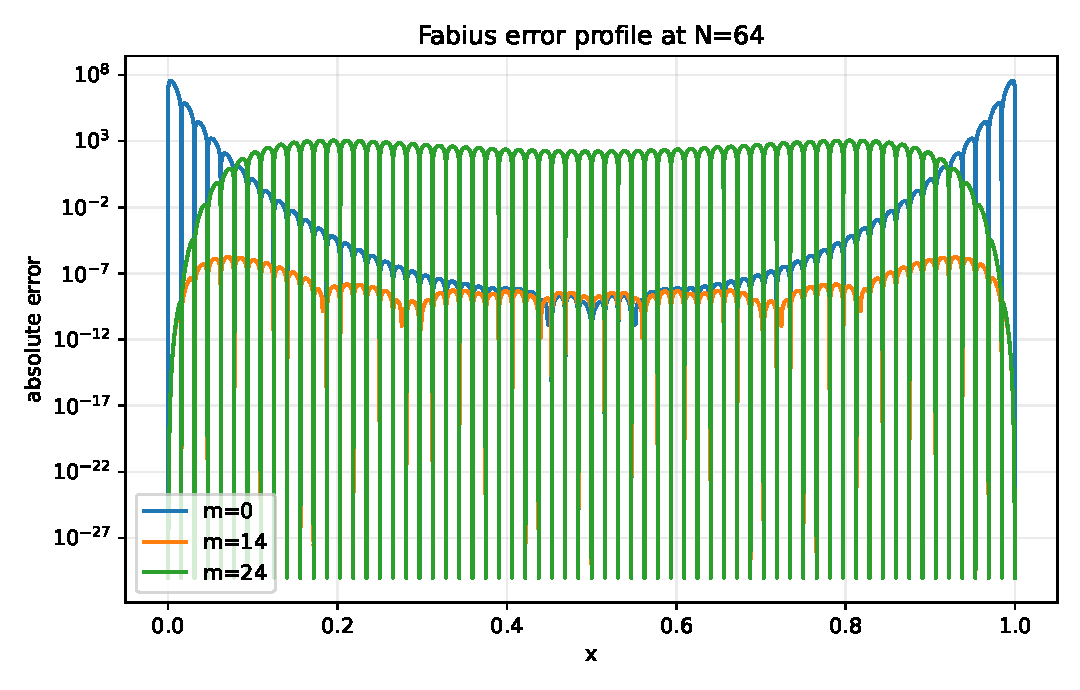
\includegraphics[width=0.88\textwidth]{figures/fabius_error_profile_N64.pdf}
\caption{Absolute error at $N=64$.  The ordinary interpolant ($m=0$) has a gigantic
boundary spike; a tuned endpoint jet ($m=14$) suppresses it; overconstraining ($m=24$)
creates a reverse instability.}
\label{fig:fabius-profile}
\end{figure}

\section{Endpoint-flat Hermite interpolation}
\label{sec:endpoint-flat}

\subsection{The constrained problem}

For $m\ge0$, seek a polynomial $P_{N,m}$ satisfying
\begin{align}
 P_{N,m}(j/N)&=F(j/N), &&0\le j\le N,\label{eq:value-conditions}\\
 P_{N,m}^{(r)}(0)&=P_{N,m}^{(r)}(1)=0,
 &&1\le r\le m.\label{eq:jet-conditions}
\end{align}
There are $N+2m+1$ scalar conditions, so the natural degree bound is $N+2m$.
A direct confluent Vandermonde solve would be both expensive and ill-conditioned.  The
flatness conditions instead permit an exact factorization.

Define the beta smoothstep
\begin{equation}
 S_m(x):=I_x(m+1,m+1)
 =\frac{(2m+1)!}{(m!)^2}\int_0^x t^m(1-t)^m\,\dd t.
 \label{eq:beta-smoothstep}
\end{equation}
It is a polynomial of degree $2m+1$ with
\begin{equation}
 S_m(0)=0,\quad S_m(1)=1,\quad
 S_m^{(r)}(0)=S_m^{(r)}(1)=0\quad(1\le r\le m),
 \label{eq:smoothstep-jets}
\end{equation}
and $S_m(1-x)=1-S_m(x)$.  Put
\begin{equation}
 W_m(x):=[x(1-x)]^{m+1}.
 \label{eq:weight}
\end{equation}

\begin{theorem}[Exact endpoint-flat factorization]
\label{thm:factorization}
There is a unique polynomial $P_{N,m}$ of degree at most $N+2m$ satisfying
\eqref{eq:value-conditions}--\eqref{eq:jet-conditions}.  It is
\begin{equation}
 P_{N,m}(x)=S_m(x)+W_m(x)Q_{N,m}(x),
 \label{eq:factorization}
\end{equation}
where $Q_{N,m}$ is the unique polynomial of degree at most $N-2$ interpolating the
interior data
\begin{equation}
 Q_{N,m}(j/N)=
 \frac{F(j/N)-S_m(j/N)}{[\frac jN(1-\frac jN)]^{m+1}},
 \qquad 1\le j\le N-1.
 \label{eq:quotient-data}
\end{equation}
For even $N$, $P_{N,m}(1-x)=1-P_{N,m}(x)$ and its actual degree is at most
$N+2m-1$.
\end{theorem}

\begin{proof}
If $P$ satisfies the endpoint values and jets, then $P-S_m$ has zeros of multiplicity
$m+1$ at both $0$ and $1$.  Hence $P-S_m=W_mQ$ for a polynomial $Q$.  The degree bound on
$P$ implies $\deg Q\le N-2$, and the interior value conditions force
\eqref{eq:quotient-data}; ordinary interpolation at $N-1$ distinct points gives uniqueness.
Conversely, \eqref{eq:factorization} has all required values and jets.  Symmetry follows by
applying uniqueness to $1-P_{N,m}(1-x)$.  Centered oddness removes the top even degree.
\end{proof}

The beta polynomial can be evaluated without special functions:
\begin{equation}
 S_m(x)=\frac{(2m+1)!}{(m!)^2}
 \sum_{r=0}^{m}(-1)^r\binom mr\frac{x^{m+r+1}}{m+r+1}.
 \label{eq:smoothstep-explicit}
\end{equation}
Thus, when $N$ is dyadic, all nodal quotient data in
\eqref{eq:quotient-data} are rational.

\subsection{Rvachev version}

For $u(x)=\upf(2x-1)$, both endpoint values are zero.  The bridge vanishes and the unique
endpoint-flat interpolant is simply
\begin{equation}
 U_{N,m}(x)=W_m(x)R_{N,m}(x),
 \label{eq:up-factorization}
\end{equation}
where $R_{N,m}$ interpolates
\begin{equation}
 R_{N,m}(j/N)=\frac{u(j/N)}{[\frac jN(1-\frac jN)]^{m+1}}.
 \label{eq:up-quotient}
\end{equation}
Since $u(1-x)=u(x)$, the quotient and interpolant are symmetric about $1/2$.

\subsection{Barycentric implementation}

For the interior nodes $j/N$, $1\le j\le N-1$, barycentric weights are proportional to
\begin{equation}
 \widetilde w_j=(-1)^{j-1}\binom{N-2}{j-1}.
 \label{eq:interior-weights}
\end{equation}
Writing $g_j$ for the quotient data, one evaluates
\begin{equation}
 Q_{N,m}(x)=
 \frac{\displaystyle\sum_{j=1}^{N-1}
       \frac{\widetilde w_jg_j}{x-j/N}}
      {\displaystyle\sum_{j=1}^{N-1}
       \frac{\widetilde w_j}{x-j/N}}.
 \label{eq:quotient-barycentric}
\end{equation}
No confluent matrix is formed.  This algorithm is exact at nodes, uses exact rational
samples, and requires only arbitrary-precision arithmetic in the off-node evaluation.

\subsection{Confluent remainder and why it is not predictive}

Let
\begin{equation}
 M=N+2m+1.
\end{equation}
The classical Hermite remainder gives, for each $x$ and some $\xi_x\in(0,1)$,
\begin{equation}
 F(x)-P_{N,m}(x)=
 \frac{F^{(M)}(\xi_x)}{M!}
 x^{m+1}(x-1)^{m+1}
 \prod_{j=1}^{N-1}\left(x-\frac jN\right).
 \label{eq:hermite-remainder}
\end{equation}
Combining this with \eqref{eq:derivative-growth} produces a formally valid but enormous
upper bound containing $2^{M(M+1)/2}$.  It cannot explain the observed cancellation.  The
right diagnostic is not a derivative supremum but the data-amplification geometry developed
next.

\section{Weighted Lebesgue geometry and two exact obstructions}
\label{sec:conditioning}

\subsection{The relevant operator norm}

Perturb only the $N-1$ interior values, keeping endpoint values and endpoint jets exact.
The perturbation of \eqref{eq:factorization} is
\begin{equation}
 \delta P(x)=W_m(x)\sum_{j=1}^{N-1}
       \frac{\delta f_j}{W_m(j/N)}\ell_j^{\rm int}(x),
 \label{eq:perturbation}
\end{equation}
where $\ell_j^{\rm int}$ is the ordinary cardinal polynomial for the interior comb.  The
corresponding pointwise and global Lebesgue functions are
\begin{align}
 \Leb_{N,m}(x)&=
 \sum_{j=1}^{N-1}\left|
   \frac{W_m(x)}{W_m(j/N)}\ell_j^{\rm int}(x)
 \right|,
 \label{eq:weighted-lebesgue}\qquad\\
 \Leb_{N,m}&=\max_{x\in[0,1]}\Leb_{N,m}(x).
 \label{eq:weighted-lebesgue-global}
\end{align}
This is a lower bound on the conditioning of any implementation of the same polynomial
operator; it is independent of the barycentric evaluation strategy.

\subsection{A gamma formula for uniform cardinal functions}

Let $y=Nx$.  For $x\in(0,1)$ not a node,
\begin{equation}
 \left|\ell_j^{\rm int}(x)\right|
 =\frac{\Gamma(y)\Gamma(N-y)|\sin\pi y|}
 {\pi|y-j|\Gamma(j)\Gamma(N-j)},
 \qquad 1\le j\le N-1.
 \label{eq:gamma-cardinal}
\end{equation}
Indeed, reflection gives
\begin{equation}
 \left|\prod_{k=1}^{N-1}(y-k)\right|
 =\frac{\Gamma(y)\Gamma(N-y)|\sin\pi y|}{\pi},
\end{equation}
and differentiation at $y=j$ gives
$\prod_{k\ne j}|j-k|=\Gamma(j)\Gamma(N-j)$.
Formula \eqref{eq:gamma-cardinal} makes the two competing modes completely explicit.

\subsection{Boundary-to-center mode}

Take $x=1/(2N)$ and the central node $j=N/2$.

\begin{proposition}[First exact cardinal obstruction]
\label{prop:A-mode}
For even $N$,
\begin{equation}
 \Leb_{N,m}\ge A_{N,m}:=A_Na_N^{m+1},
 \label{eq:A-mode}
\end{equation}
where
\begin{align}
 A_N&=
 \frac{\Gamma(N-\tfrac12)}
 {\sqrt\pi\,(\tfrac N2-\tfrac12)\Gamma(N/2)^2},
 &a_N&=\frac{2N-1}{N^2}.
 \label{eq:A-components}
\end{align}
Moreover,
\begin{equation}
 A_N\sim \frac{2^N}{\pi\sqrt2\,N},
 \qquad
 A_{N,m}\sim
 \frac{2^{N+m+1}}{\pi\sqrt2\,N^{m+2}}
 \quad(m\ \text{fixed}).
 \label{eq:A-asymptotic}
\end{equation}
\end{proposition}

\begin{proof}
Keep only the $j=N/2$ term in \eqref{eq:weighted-lebesgue}.  Formula
\eqref{eq:gamma-cardinal} at $y=1/2$ gives $A_N$.  The weight ratio is
\[
 \frac{x(1-x)}{(1/2)(1/2)}=\frac{2N-1}{N^2}=a_N.
\]
Stirling's formula yields \eqref{eq:A-asymptotic}.
\end{proof}

For every fixed $m$, the first mode is exponential.  Endpoint flatness of fixed order can
delay the Runge transition but cannot change its asymptotic character.

\subsection{Center-to-boundary mode}

Now take $x=1/2+1/(2N)$ and the near-boundary node $j=1$.

\begin{proposition}[Second exact cardinal obstruction]
\label{prop:B-mode}
For even $N$,
\begin{equation}
 \Leb_{N,m}\ge B_{N,m}:=B_Nb_N^{m+1},
 \label{eq:B-mode}
\end{equation}
where
\begin{align}
 B_N&=\frac{\Gamma(N/2-\tfrac12)^2}{\pi\Gamma(N-1)},
 &b_N&=\frac{N+1}{4}.
 \label{eq:B-components}
\end{align}
Moreover,
\begin{equation}
 B_N\sim 2^{2-N}\sqrt{\frac{2}{\pi N}}.
 \label{eq:B-asymptotic}
\end{equation}
\end{proposition}

\begin{proof}
At $y=N/2+1/2$ and $j=1$, \eqref{eq:gamma-cardinal} reduces to $B_N$ because
$\Gamma(N/2+1/2)=(N/2-1/2)\Gamma(N/2-1/2)$.  The weight ratio is
\[
 \frac{(\frac12+\frac1{2N})(\frac12-\frac1{2N})}
 {(\frac1N)(1-\frac1N)}=\frac{N+1}{4}=b_N.
\]
Stirling gives \eqref{eq:B-asymptotic}.
\end{proof}

The second mode is tiny at $m=0$ but grows as approximately $(N/4)^m$.  It is the precise
mechanism behind the overconstrained blow-up.

\subsection{The logarithmically thin balance window}

Equating the exact bounds gives a distinguished real jet order.

\begin{definition}[Two-mode balance order]
\label{def:balance}
For $N>4$, define
\begin{equation}
 m_{\rm bal}(N)+1=
 \frac{\log(A_N/B_N)}{\log(b_N/a_N)}.
 \label{eq:balance-order}
\end{equation}
\end{definition}

\begin{proposition}[Asymptotic balance law]
\label{prop:balance-asymptotic}
As $N\to\infty$ through powers of two,
\begin{equation}
 m_{\rm bal}(N)=\frac{N\log2}{\log N}
 \left(1+\bigO\!\left(\frac1{\log N}\right)\right).
 \label{eq:balance-asymptotic}
\end{equation}
The leading boundary-suppression and reverse-amplification thresholds are
\begin{align}
 m_-(N)+1&\sim\frac{N\log2}{\log(N/2)},
 \label{eq:m-lower}\\
 m_+(N)+1&\sim\frac{N\log2}{\log(N/4)},
 \label{eq:m-upper}
\end{align}
and
\begin{equation}
 m_+(N)-m_-(N)
 \sim\frac{N(\log2)^2}{(\log N)^2}.
 \label{eq:window-width}
\end{equation}
\end{proposition}

\begin{proof}
Insert \eqref{eq:A-asymptotic} and \eqref{eq:B-asymptotic} into
\eqref{eq:balance-order}.  The numerator is $2N\log2+\bigO(\log N)$ and the denominator is
$2\log N+\bigO(1)$.  Equations \eqref{eq:m-lower} and \eqref{eq:m-upper} follow by
separately balancing the exponential parts of $A_{N,m}$ and $B_{N,m}$ against one.  Their
difference is an elementary expansion of the reciprocal logarithms.
\end{proof}

\begin{table}[htbp]
\centering
\caption{Exact two-mode balance order and the best tested jet order.  The $N=8$ Fabius
minimum is a small-degree anomaly; from $N=16$ onward the prediction is close.}
\label{tab:balance}
\begin{tabular}{rrrr}
\toprule
$N$ & $m_{\rm bal}$ & best tested $m$ for $F$ & best tested $m$ for $u$ \\
\midrule
8   & 2.293  & 6  & 4 \\
16  & 4.106  & 5  & 5 \\
32  & 7.163  & 8  & 8 \\
64  & 12.415 & 14 & 14 \\
128 & 21.573 & 23 (selected scan) & --- \\
256 & 37.758 & --- & --- \\
\bottomrule
\end{tabular}
\end{table}

For a fixed available jet budget $m$, the leading inversion of
$m\sim N\log2/\log N$ is
\begin{equation}
 N_{\max}(m)\sim
 -\frac{m}{\log2}
 W_{-1}\!\left(-\frac{\log2}{m}\right),
 \label{eq:lambert-budget}
\end{equation}
where $W_{-1}$ is the lower real branch of Lambert's function.  This is a direct bridge
between the interpolation problem and the lower-branch Lambert-$W$ machinery already
central in the endpoint asymptotics of $F$.

\subsection{No endpoint-jet sequence stabilizes the operator}

The two special modes explain practical tuning, but by themselves their balanced common
value can become small.  A third, entropy-scale cardinal mode proves a stronger result.
Let
\begin{equation}
 \Hbin(\theta)=-\theta\log\theta-(1-\theta)\log(1-\theta)
\end{equation}
be the binary entropy in natural logarithms.

\begin{lemma}[Interior entropy growth]
\label{lem:entropy-cardinal}
Let $N$ be divisible by $4$, take
$x_N=1/4+1/(2N)$ and $j=N/2$.  Then
\begin{equation}
 \log\left|\ell_{N/2}^{\rm int}(x_N)\right|
 =N\bigl(\log2-\Hbin(1/4)\bigr)+\bigO(\log N).
 \label{eq:entropy-growth}
\end{equation}
Furthermore,
\begin{equation}
 \frac{x_N(1-x_N)}{1/4}\longrightarrow\frac34.
 \label{eq:entropy-weight}
\end{equation}
\end{lemma}

\begin{proof}
Apply Stirling's formula to \eqref{eq:gamma-cardinal}.  The exponential part of the gamma
quotient is the difference between the entropy rates at $j/N=1/2$ and $x_N\to1/4$.
The weight ratio is immediate.
\end{proof}

\begin{theorem}[Universal endpoint-flat instability]
\label{thm:universal-instability}
There exist absolute constants $c,C>0$ and $N_0$ such that, for every dyadic
$N\ge N_0$ and every integer $m\ge0$,
\begin{equation}
 \Leb_{N,m}\ge C\e^{cN}.
 \label{eq:universal-instability}
\end{equation}
In particular, no sequence $m=m_N$ makes the endpoint-flat global interpolation operators
subexponentially conditioned on the complete dyadic comb.
\end{theorem}

\begin{proof}
Set $\alpha=\log2-\Hbin(1/4)>0$.  Choose a sufficiently small constant
$\varepsilon>0$.

If $m\le\varepsilon N$, keep the $j=N/2$ term at $x_N$ from
\cref{lem:entropy-cardinal}.  Its logarithm is
\[
 N\alpha+m\log(3/4+o(1))+\bigO(\log N),
\]
which is at least $c_1N$ by the choice of $\varepsilon$.

If $m>\varepsilon N$, use the exact lower bound \eqref{eq:B-mode}.  By
\eqref{eq:B-asymptotic},
\[
 \log B_{N,m}
 \ge -N\log2+\varepsilon N\log(N/4)+\bigO(\log N),
\]
which exceeds $c_2N$ for all sufficiently large $N$ (indeed it is eventually of order
$N\log N$).  Taking $c=\min(c_1,c_2)$ and absorbing finitely many prefactors into $C$
proves the claim.
\end{proof}

\begin{corollary}
For each fixed $m$, the endpoint-flat interpolation operator is exponentially unstable;
for every linear growth law $m\ge\varepsilon N$, it is eventually superexponentially
unstable in $N$.
\end{corollary}

This theorem is compatible with the spectacular actual errors in
\cref{sec:numerics}: a large operator norm need not be realized by the highly correlated,
self-similar Fabius samples.  It does mean that data noise, rounding, or a generic smooth
perturbation can destroy the cancellation.

\section{Numerical experiments}
\label{sec:numerics}

\subsection{Protocol}

The accompanying \path{numerical_experiments.py} implements
\eqref{eq:V-recurrence}--\eqref{eq:bit-recursion} with Python's exact
\texttt{Fraction}.  Interpolants are evaluated by scaled barycentric formulas in
\texttt{mpmath}, generally at $120$ to $300$ decimal digits.  Precision was increased
until every displayed digit stabilized.  Error maxima are sampled on all dyadic points of
a stated fine grid, not on a random subset.  The program also verifies symmetry, nodal
reproduction, beta-bridge endpoint values, and several known small dyadic values before
running the experiments.

The experiments distinguish two notions:
\begin{itemize}
\item \emph{actual error}, obtained from the exact Fabius or Rvachev data;
\item \emph{worst-case amplification}, measured by the weighted Lebesgue function.
\end{itemize}
Conflating these notions would hide the most interesting result.

\subsection{Fabius endpoint jets}

\begin{table}[htbp]
\centering
\caption{Ordinary and best tested endpoint-flat interpolation errors for $F$ on a grid of
mesh $2^{-12}$.}
\label{tab:fabius-best}
\begin{tabular}{rrrrr}
\toprule
$N$ & ordinary error & best tested $m$ & best tested error & improvement factor \\
\midrule
8  & $9.48677\times10^{-3}$ & 6  & $2.09066\times10^{-4}$ & $4.54\times10^1$ \\
16 & $3.79662\times10^{-3}$ & 5  & $2.73408\times10^{-5}$ & $1.39\times10^2$ \\
32 & $4.98935$               & 8  & $7.62257\times10^{-7}$ & $6.55\times10^6$ \\
64 & $3.58889\times10^{7}$  & 14 & $1.77661\times10^{-6}$ & $2.02\times10^{13}$ \\
\bottomrule
\end{tabular}
\end{table}

At $N=64$, selected values make the reversal explicit:
\begin{equation}
\begin{array}{c|rrrrrrrr}
m&0&8&10&12&14&16&20&24\\ \hline
\lVert P_{64,m}-F\rVert_\infty
&3.59\!\times\!10^7&4.76\!\times\!10^{-3}&1.56\!\times\!10^{-4}
&8.30\!\times\!10^{-6}&1.78\!\times\!10^{-6}&7.80\!\times\!10^{-5}
&4.73&1.13\!\times\!10^3
\end{array}
\label{eq:N64-selected}
\end{equation}
The selected $N=128$ scan gave errors $1.57\times10^{-1}$, $3.36\times10^{-2}$,
$7.88\times10^{-3}$, $3.98\times10^{-3}$, and $1.70\times10^{-2}$ at
$m=20,21,22,23,24$, respectively, against an ordinary error
$3.84\times10^{22}$.

\begin{figure}[htbp]
\centering
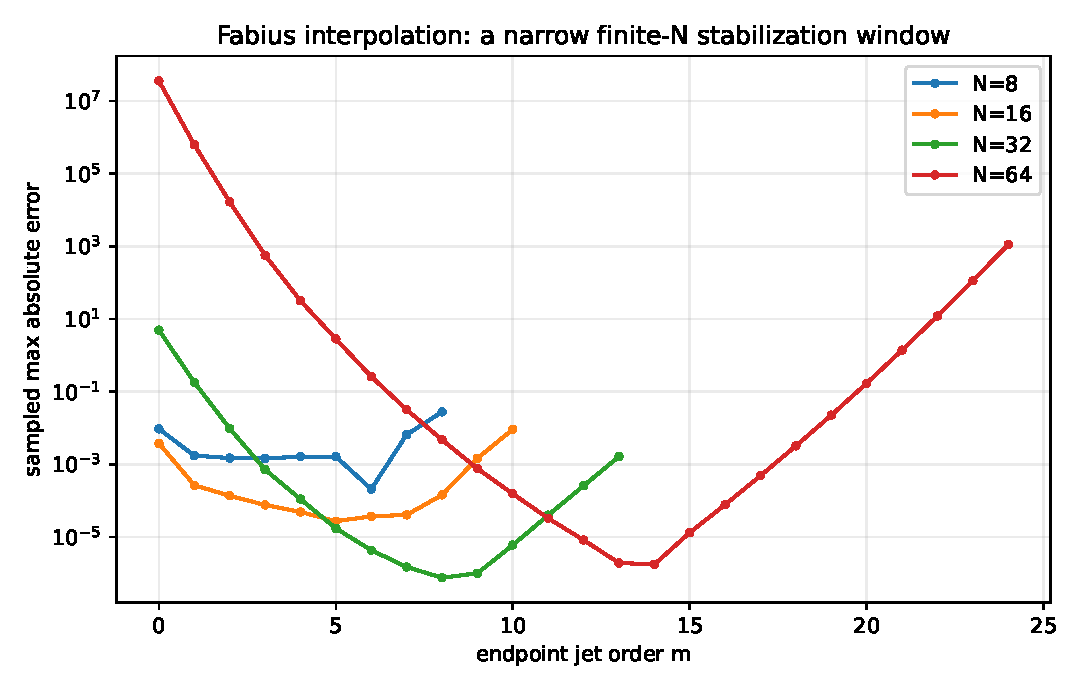
\includegraphics[width=0.88\textwidth]{figures/fabius_error_vs_jet.pdf}
\caption{Fabius error versus endpoint jet order.  Every sufficiently resolved curve is
U-shaped: ordinary Runge growth is first suppressed, then a reverse mode appears.}
\label{fig:fabius-error-vs-m}
\end{figure}

\subsection{Rvachev endpoint jets}

\begin{table}[htbp]
\centering
\caption{Ordinary and best tested endpoint-flat interpolation errors for
$u(x)=\upf(2x-1)$.}
\label{tab:up-best}
\begin{tabular}{rrrrr}
\toprule
$N$ & ordinary error & best tested $m$ & best tested error & improvement factor \\
\midrule
8  & $2.02170\times10^{-1}$ & 4  & $1.33916\times10^{-2}$ & $1.51\times10^1$ \\
16 & $1.96934\times10^{-1}$ & 5  & $6.50226\times10^{-4}$ & $3.03\times10^2$ \\
32 & $4.49719\times10^{2}$  & 8  & $4.08484\times10^{-5}$ & $1.10\times10^7$ \\
64 & $1.04564\times10^{10}$ & 14 & $6.19248\times10^{-4}$ & $1.69\times10^{13}$ \\
\bottomrule
\end{tabular}
\end{table}

The same optimal orders for $N=16,32,64$ are notable because $u$ uses no beta bridge.
This supports the interpretation that the order is controlled primarily by node geometry
and endpoint multiplicity, while the detailed target determines how completely the large
modes cancel.

\begin{figure}[htbp]
\centering
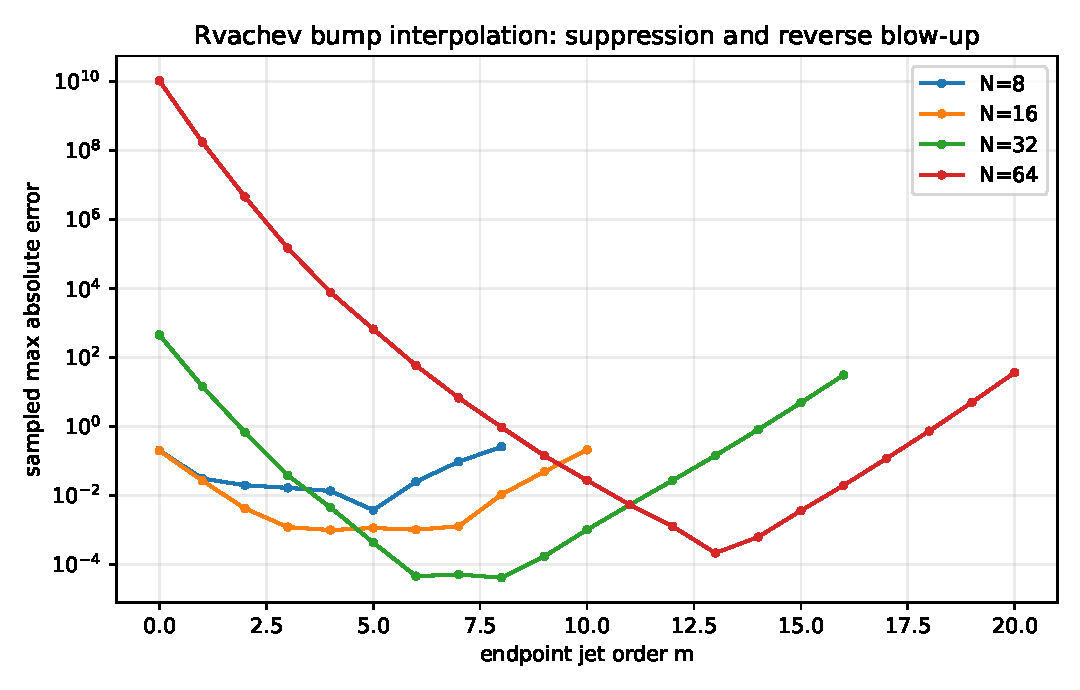
\includegraphics[width=0.88\textwidth]{figures/up_error_vs_jet.pdf}
\caption{Endpoint-flat interpolation of the centered Rvachev bump.}
\label{fig:up-error-vs-m}
\end{figure}

\subsection{Actual accuracy versus operator conditioning}

At $N=64$, a mesh-$2^{-11}$ scan of \eqref{eq:weighted-lebesgue-global} gives
\begin{equation}
\begin{array}{c|rrrrrrrr}
m&0&8&10&12&14&16&20&24\\ \hline
\Leb_{64,m}
&4.40\!\times\!10^{16}&6.40\!\times\!10^{6}&2.20\!\times\!10^{5}
&1.29\!\times\!10^{4}&2.83\!\times\!10^{3}&4.37\!\times\!10^{4}
&8.46\!\times\!10^{7}&5.49\!\times\!10^{11}.
\end{array}
\label{eq:lebesgue-selected}
\end{equation}
The practical Fabius optimum $m=14$ therefore still has a worst-case amplification of
about $2825$.  The target's self-similar residual data happen to avoid the dangerous sign
pattern.

\begin{figure}[htbp]
\centering
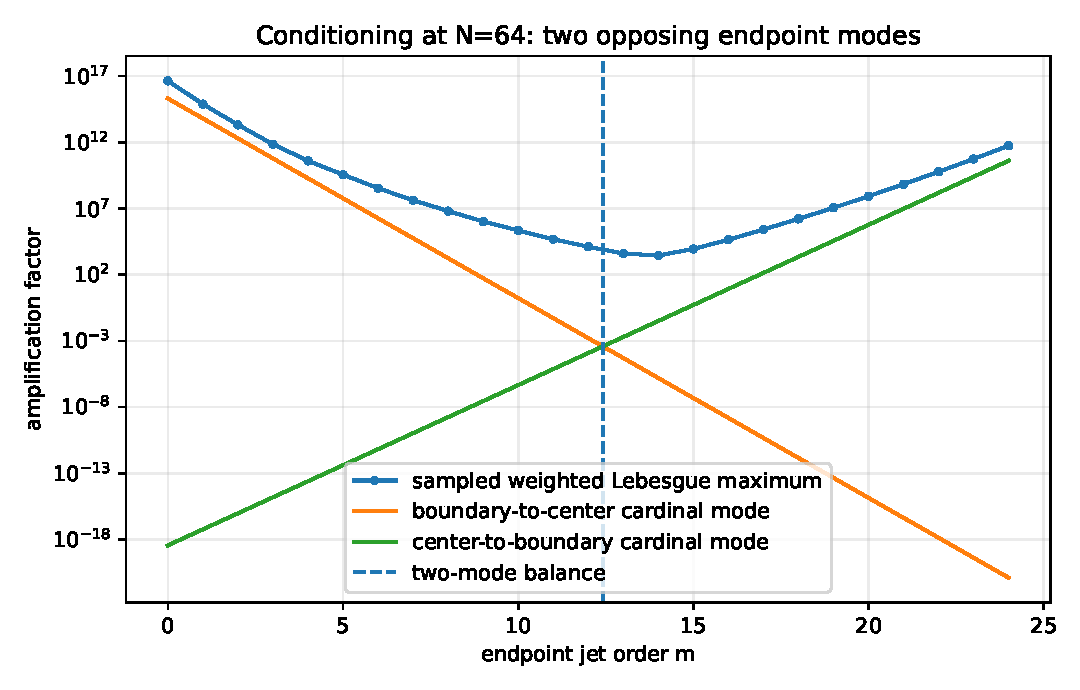
\includegraphics[width=0.88\textwidth]{figures/conditioning_window_N64.pdf}
\caption{The sampled weighted Lebesgue maximum and the two exact cardinal lower modes at
$N=64$.  Their crossing predicts the useful finite-$N$ window.}
\label{fig:conditioning-window}
\end{figure}

\subsection{Why fixing derivatives at every node is worse}

One might instead match both $F(x_j)$ and $F'(x_j)$ at all $N+1$ nodes, producing the
standard first-order Hermite polynomial of degree at most $2N+1$.  With ordinary cardinal
functions $\ell_j$ it is
\begin{equation}
 H_N(x)=\sum_{j=0}^{N}
 \left[
  \bigl(1-2\ell'_j(x_j)(x-x_j)\bigr)\ell_j(x)^2F(x_j)
  +(x-x_j)\ell_j(x)^2F'(x_j)
 \right].
 \label{eq:all-node-hermite}
\end{equation}
The dyadic derivatives are exact because
\begin{equation}
 F'(j/N)=2F\!\left(2\min(j/N,1-j/N)\right).
\end{equation}

\begin{table}[htbp]
\centering
\caption{First-derivative Hermite interpolation at every dyadic node.}
\label{tab:all-node-hermite}
\begin{tabular}{rrr}
\toprule
$N$ & degree bound & sampled maximum error \\
\midrule
4  & 9   & $1.14814\times10^{-2}$ \\
8  & 17  & $3.73583\times10^{-3}$ \\
16 & 33  & $2.27198$ \\
32 & 65  & $1.53809\times10^{7}$ \\
64 & 129 & $1.35218\times10^{23}$ \\
\bottomrule
\end{tabular}
\end{table}

The squared cardinal functions in \eqref{eq:all-node-hermite} effectively square the
already dangerous equispaced geometry, while the extra degree provides more room for
oscillation.  Higher derivative information is therefore not intrinsically stabilizing;
\emph{where} it is imposed matters more than the fact that it is exact.

\begin{figure}[htbp]
\centering
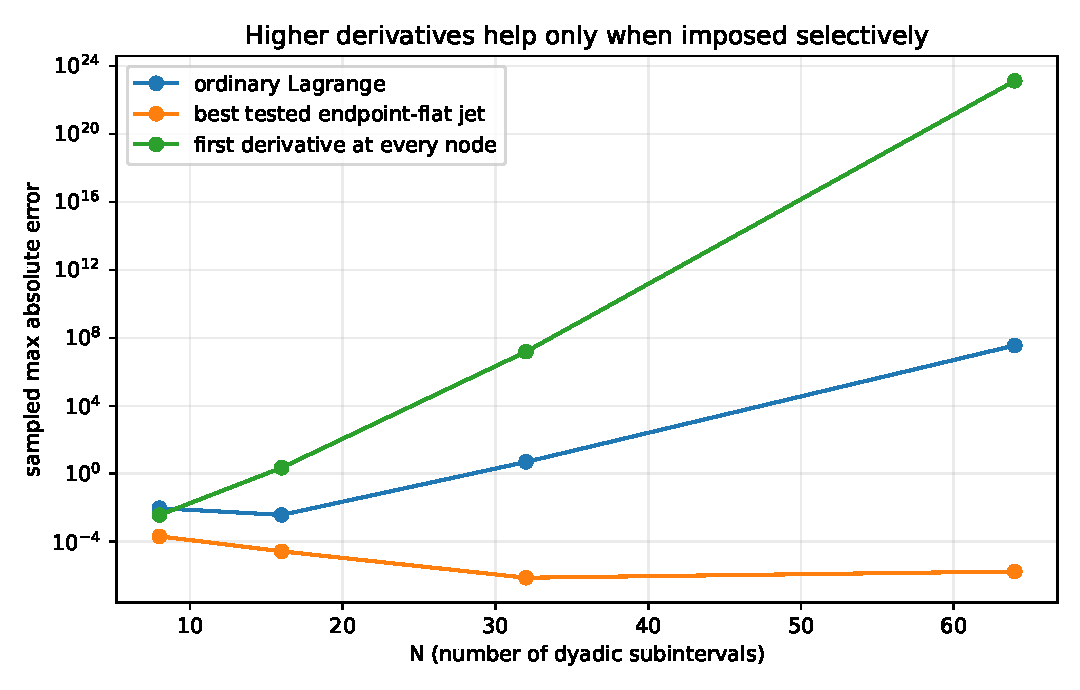
\includegraphics[width=0.88\textwidth]{figures/method_comparison.pdf}
\caption{Ordinary Lagrange, best tested endpoint-flat interpolation, and all-node first
Hermite interpolation.}
\label{fig:method-comparison}
\end{figure}

\subsection{Exact endpoint derivative defect}

Equation \eqref{eq:endpoint-derivative} was evaluated as a reduced rational number.  The
following values show the scale; the sign is irregular.

\begin{table}[htbp]
\centering
\caption{Exact endpoint derivative defect of the ordinary Fabius interpolant.}
\label{tab:derivative-defect}
\begin{tabular}{rrrr}
\toprule
$N$ & sign & $\log_2|(L_NF)'(0)|$ & $N-\log_2|(L_NF)'(0)|$ \\
\midrule
16   & $+$ & $-0.681$ & $16.681$ \\
32   & $-$ & $10.816$ & $21.184$ \\
64   & $+$ & $34.823$ & $29.177$ \\
128  & $-$ & $85.942$ & $42.058$ \\
256  & $-$ & $206.287$ & $49.713$ \\
512  & $-$ & $450.491$ & $61.509$ \\
1024 & $+$ & $949.989$ & $74.011$ \\
2048 & $+$ & $1957.083$ & $90.917$ \\
4096 & $-$ & $3992.945$ & $103.055$ \\
8192 & $-$ & $8070.574$ & $121.426$ \\
\bottomrule
\end{tabular}
\end{table}

The defect is a particularly clean observable because the true derivative is exactly zero.
It is also a binomial transform of exact dyadic values, making it a natural meeting point of
uniform-node interpolation and the project's Thue--Morse/$q$-binomial arithmetic.

\begin{figure}[htbp]
\centering
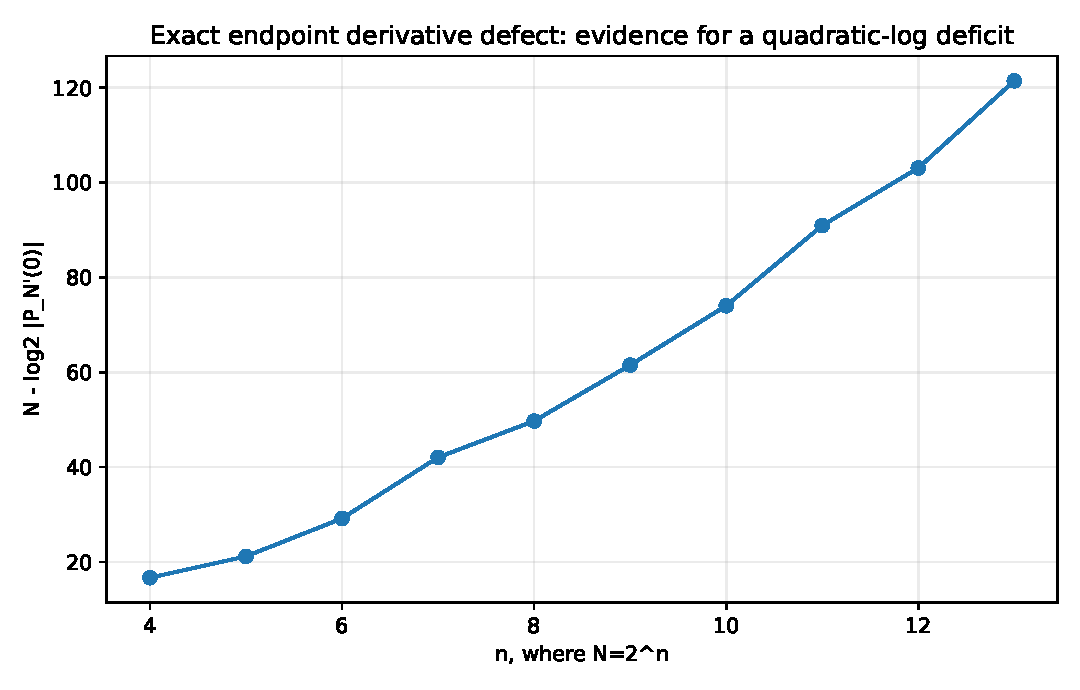
\includegraphics[width=0.88\textwidth]{figures/endpoint_derivative_deficit.pdf}
\caption{The binary deficit $N-\log_2|(L_NF)'(0)|$.  The data are consistent with a
quadratic function of $\log_2N$ plus lower-order oscillation.}
\label{fig:derivative-deficit}
\end{figure}

\section{Connections with the project's $q$-series and Thue--Morse structures}
\label{sec:q-connections}

\subsection{A mixed binomial transform}

At uniform nodes, the interpolation weights are the ordinary Pascal row
$(-1)^j\binom Nj$---a $q=1$ object.  The dyadic Fabius values are governed by
$q=1/2$ Pochhammer products and Gaussian binomial coefficients in the audited corpus.
The endpoint defect
\begin{equation}
 D_N=N\sum_{j=1}^{N}(-1)^{j+1}\binom Nj\frac{F(j/N)}j
 \label{eq:mixed-transform}
\end{equation}
is therefore a mixed $q=1$/$q=1/2$ transform.  It deserves study as an arithmetic object
in its own right.

Writing $1/j=\int_0^1t^{j-1}\,\dd t$ gives
\begin{equation}
 \frac{D_N}{N}
 =\int_0^1\sum_{j=1}^{N}(-1)^{j+1}\binom NjF(j/N)t^{j-1}\,\dd t.
 \label{eq:derivative-integral}
\end{equation}
This representation may permit a saddle analysis after inserting an exact dyadic-value
formula.  The alternating Pascal row has the same finite-difference cancellation that
underlies Prouhet identities, but the nonpolynomial Fabius samples leave a small, highly
structured residue.

\subsection{Newton coefficients and Prouhet cancellation}

The coefficients $\Delta^kF(0)$ in \eqref{eq:newton-ordinary} annihilate polynomial trends
of degree below $k$.  For $N=2^n$, the dyadic sample vector itself has recursive blocks
controlled by binary digit patterns.  It is plausible that the observed sign changes and
the sublinear deficit in \cref{tab:derivative-defect} arise from a competition between:
\begin{itemize}
\item the entropy concentration of the Pascal row near $j=N/2$;
\item exact Prouhet-type cancellation among dyadic blocks;
\item the lower-Lambert endpoint scale governing $F(j/N)$ for small $j$;
\item a residual log-periodic phase inherited from the endpoint asymptotics.
\end{itemize}
A rigorous asymptotic for \eqref{eq:mixed-transform} would connect several currently
separate parts of the project.

\subsection{Bell and Bernoulli polynomials in refined balance laws}

The leading balance law \eqref{eq:balance-asymptotic} uses only first-order Stirling
expansions.  All higher corrections to $\log A_N$, $\log B_N$, $\log a_N$, and
$\log b_N$ are explicit Bernoulli-polynomial series.  Reversion of
\eqref{eq:balance-order} can be organized with complete Bell polynomials, exactly as in the
project's all-orders Lambert-$W$ endpoint expansions.  Thus one can obtain
\begin{equation}
 m_{\rm bal}(N)
 \sim \frac{N\log2}{\log N}
 \left(1+\frac{c_1}{\log N}
 +\frac{c_2(\log\log N)}{(\log N)^2}+\cdots\right),
 \label{eq:balance-all-orders}
\end{equation}
with computable coefficients.  The exact formula \eqref{eq:balance-order} is already easy
to evaluate, so the principal value of \eqref{eq:balance-all-orders} is conceptual and
formal: it places the interpolation window in the same asymptotic calculus as the Fabius
endpoint.

\section{What has and has not been proved about Runge divergence}
\label{sec:runge-status}

The operator instability is proved in \cref{thm:universal-instability}.  That theorem says
there exist value perturbations whose interpolants grow exponentially, for every choice of
endpoint jet order.  It does not by itself prove that the \emph{particular deterministic
sequence} $L_NF$ diverges in supremum norm as $N\to\infty$.

For $F$, the numerical evidence is nevertheless overwhelming:
\begin{itemize}
\item direct exact-sample errors grow from $4.99$ to $3.59\times10^7$ to
      $3.84\times10^{22}$ as $N$ goes from $32$ to $64$ to $128$;
\item the endpoint derivative defect is exact and nearly $2^N$ on a logarithmic scale;
\item the spike location scales like $x\asymp1/N$;
\item increasing precision and refining the test grid leave the results unchanged.
\end{itemize}
A proof of the endpoint derivative conjecture below would immediately imply nonuniform
convergence.  With a quantitative Markov inequality, it would also force a large supremum
norm of the interpolant in a boundary interval.

\section{Conjectures and frontier problems}
\label{sec:conjectures}

\begin{conjecture}[Fabius Runge divergence]
\label{conj:runge}
For $N=2^n$,
\begin{equation}
 \lVert L_NF-F\rVert_\infty\longrightarrow\infty.
\end{equation}
More strongly, $\log_2\lVert L_NF\rVert_\infty=N-o(N)$ along a subsequence.
\end{conjecture}

\begin{conjecture}[Endpoint derivative law]
\label{conj:derivative}
There are positive constants $c_1,c_2$ such that
\begin{equation}
 N-c_2(\log_2N)^2
 \le \log_2|(L_NF)'(0)|
 \le N-c_1(\log_2N)^2
 \label{eq:derivative-conjecture}
\end{equation}
for all sufficiently large dyadic $N$ outside a possible sparse zero set.  After subtracting
the principal quadratic-log term, the remainder contains a bounded or slowly growing
log-periodic component related to the endpoint phase of $F$.
\end{conjecture}

The sign data suggest that a clean one-term asymptotic may require phase locking in
$n=\log_2N$, analogous to the phase-locked Richardson procedures already present in the
repository.

\begin{conjecture}[Optimal actual jet order]
\label{conj:optimal-m}
Let $m_F(N)$ and $m_u(N)$ minimize the true supremum errors of $P_{N,m}$ and $U_{N,m}$.
Then
\begin{equation}
 m_F(N)=m_{\rm bal}(N)+\bigO\!\left(\frac{\log N}{\log\log N}\right),
 \qquad
 m_u(N)=m_{\rm bal}(N)+\bigO\!\left(\frac{\log N}{\log\log N}\right).
 \label{eq:optimal-m-conjecture}
\end{equation}
A stronger and numerically plausible version replaces the error term by $\bigO(1)$ along a
phase-locked dyadic subsequence.
\end{conjecture}

\begin{conjecture}[Boundary-layer profile]
\label{conj:boundary-profile}
There exist normalizations $A_N$, $B_N$ and a subsequence of dyadic $N$ such that the
ordinary interpolation error has a nontrivial scaled limit
\begin{equation}
 A_N\bigl((L_NF)(\xi/N)-F(\xi/N)\bigr)
 \longrightarrow \mathcal E(\xi)
 \label{eq:boundary-profile-conjecture}
\end{equation}
locally for $\xi>0$.  The profile $\mathcal E$ is governed jointly by the entropy saddle of
the uniform cardinal functions and the lower-Lambert endpoint asymptotic of $F$.
\end{conjecture}

\begin{problem}[Arithmetic of the mixed transform]
Determine a closed form, recurrence, $2$-adic valuation law, or Mahler equation for
$D_{2^n}$ in \eqref{eq:mixed-transform}.  Even a sharp upper and lower bound of the form
\eqref{eq:derivative-conjecture} would settle the most basic Fabius-specific Runge question.
\end{problem}

\begin{problem}[Noise threshold]
For tuned $m=m_{\rm bal}(N)$, quantify the largest relative perturbation of the exact dyadic
samples that preserves the observed Fabius accuracy.  The crude threshold
$\Leb_{N,m}^{-1}$ is pessimistic; the relevant structured condition number should project
noise onto the self-similar residual subspace.
\end{problem}

\section{Stable replacements for a global equispaced polynomial}
\label{sec:alternatives}

The negative operator theorem does not make the dyadic comb unusable.  It says only that
using all samples in one high-degree polynomial is the wrong global representation.
Several replacements preserve the exact dyadic arithmetic.

\subsection{Piecewise dyadic Hermite splines}

Divide $[0,1]$ into dyadic blocks and use low-degree Hermite pieces.  Derivatives at dyadic
nodes are again exact Fabius values at a finer scale.  One can enforce $C^r$ continuity and
retain strict locality.  Because the polynomial degree stays fixed while the block size
shrinks, there is no global Runge mechanism.  This is the most direct practical method.

\subsection{Constrained least squares with degree below $N$}

The impossibility theorem of Platte, Trefethen, and Kuijlaars shows that stable exponential
convergence from equispaced samples is unavailable, but stable root-exponential convergence
is compatible with a polynomial degree of order $\sqrt N$.  For Fabius data, solve a
weighted least-squares problem of degree $d\asymp\sqrt N$ while imposing exact endpoint
flatness.  The beta-factorization still applies, but $Q$ is fitted rather than interpolated.
Oversampling converts the dangerous square system into a stable rectangular one.

\subsection{Mapped Chebyshev and fake-node methods}

Map the dyadic samples to approximate Chebyshev locations, or construct a polynomial in a
nonlinear coordinate whose pullback nodes are near-Chebyshev.  The map should respect
$x\leftrightarrow1-x$ and the boundary flatness.  A particularly natural family uses a
Lambert coordinate fitted to the known endpoint scale, rather than a generic Kosloff--Tal-
Ezer map.

\subsection{Rational and Floater--Hormann interpolation}

Local-degree rational barycentric formulas on equispaced nodes have much smaller Lebesgue
constants and no polynomial endpoint catastrophe.  Endpoint derivative constraints can be
incorporated by rational Hermite formulas or by applying the rational interpolant to the
quotient in \eqref{eq:factorization}.  Poles must be monitored, but the method is a better
candidate than global all-node Hermite interpolation.

\subsection{Self-similar multiresolution bases}

The infinite sinc product and Rvachev refinement equation suggest a basis adapted to the
function rather than to generic algebraic polynomials.  A multiresolution expansion in
scaled translates of $\upf$ would represent the dyadic recursion exactly and turn
interpolation into a sparse refinement problem.  This direction is closest to the intrinsic
geometry of the target.

\subsection{Inverse Fabius interpolation}

Direct polynomial interpolation of $F^{-1}$ near $0$ and $1$ is even more delicate because
the inverse has singular derivatives.  The lower-Lambert variable should be used first:
interpolate the slowly varying correction after removing the known asymptotic inverse.  The
present endpoint-flat polynomial is not the right tool for the inverse problem.

\section{Lean formalization program}
\label{sec:lean}

The core new results are well suited to formalization because they separate algebraic,
finite, and asymptotic layers.

\begin{enumerate}
\item \textbf{Algebraic factorization.}  Define the beta smoothstep as the finite polynomial
      \eqref{eq:smoothstep-explicit}; prove endpoint jets, symmetry, divisibility by
      $x^{m+1}(1-x)^{m+1}$, and uniqueness of \cref{thm:factorization}.
\item \textbf{Uniform cardinal formula.}  First prove finite-product versions of the two
      special cardinal evaluations.  The gamma formulas can be added later; the exact
      products already suffice for the lower bounds.
\item \textbf{Two obstruction theorems.}  Formalize \cref{prop:A-mode,prop:B-mode} with
      factorials and central binomial coefficients.  Translate to gamma notation as a
      corollary.
\item \textbf{Universal instability.}  Use explicit Stirling bounds for factorials rather
      than asymptotic notation.  The dichotomy $m\le\varepsilon N$ versus
      $m>\varepsilon N$ is elementary once the finite cardinal products are available.
\item \textbf{Exact computational certificates.}  Import selected rational error values for
      small $N$ as kernel-checked examples, not as theorems about continuum maxima.
\item \textbf{Endpoint defect.}  Prove \eqref{eq:endpoint-derivative} from the barycentric
      basis and connect it to the existing finite-difference and dyadic-value modules.
\end{enumerate}

A useful module decomposition would be
\begin{center}
\begin{tabularx}{\textwidth}{>{\raggedright\arraybackslash}p{0.36\textwidth}X}
\toprule
Module & Contents \\
\midrule
\path{DyadicCombLagrange} & nodes, barycentric weights, symmetry, Newton form \\
\path{EndpointFlatHermite} & beta bridge, factorization, uniqueness \\
\path{WeightedLebesgue} & perturbation operator and cardinal functions \\
\path{DyadicCombObstructions} & exact $A$ and $B$ modes \\
\path{DyadicCombInstability} & exponential lower-bound theorem \\
\path{FabiusInterpolationDefect} & exact endpoint derivative transform \\
\bottomrule
\end{tabularx}
\end{center}

\section{Reproducibility and archive contents}
\label{sec:reproducibility}

The accompanying archive contains:
\begin{itemize}
\item this LaTeX source and the compiled PDF;
\item \path{numerical_experiments.py}, with detailed comments and command-line tasks;
\item \path{requirements.txt};
\item all CSV outputs under \path{data};
\item all vector figures under \path{figures};
\item \path{README.md} with exact reproduction commands;
\item \path{SHA256SUMS} for integrity checking.
\end{itemize}

The principal commands are:
\begin{lstlisting}[style=python]
python numerical_experiments.py --task smoke
python numerical_experiments.py --task fabius --N 64 --m-start 0 --m-end 24 \
    --grid-level 12 --output data/fabius_N64.csv
python numerical_experiments.py --task up --N 64 --m-start 0 --m-end 20 \
    --grid-level 12 --output data/up_N64.csv
python numerical_experiments.py --task lebesgue --N 64 --m-start 0 --m-end 24 \
    --grid-level 11 --output data/lebesgue_N64.csv
python numerical_experiments.py --task figures \
    --data-dir data --figure-dir figures
\end{lstlisting}

\section{Conclusions}
\label{sec:conclusion}

Global equispaced interpolation of the Fabius and Rvachev functions is a particularly clean
laboratory for Runge instability.  The target is infinitely smooth, its dyadic samples are
exact, its endpoints are flat to every order, and yet ordinary interpolation blows up.
This removes several common numerical excuses and exposes the node geometry directly.

Endpoint-flat Hermite constraints do something genuinely remarkable: at $N=64$ they turn a
$10^7$ error into a $10^{-6}$ error.  But they do so only in a narrow order window.  The
exact factorization by $[x(1-x)]^{m+1}$ reveals two opposing cardinal modes; their balance
predicts $m\asymp N/\log N$ and explains both the suppression and the reversal.  A separate
entropy mode proves that no order sequence stabilizes arbitrary data.

The most promising theoretical frontier is now sharply posed: explain why the special
Fabius residual vector cancels an exponentially ill-conditioned operator so efficiently,
and derive the endpoint derivative transform asymptotically from the existing
Thue--Morse, $q$-binomial, and Lambert-$W$ machinery.  The most promising practical route is
not a still higher global polynomial, but a local or oversampled representation adapted to
the dyadic self-similarity.

\appendix

\section{Derivation of the interior cardinal formula}
\label{app:cardinal}

Let
\begin{equation}
 \omega_N(y)=\prod_{k=1}^{N-1}(y-k).
\end{equation}
For noninteger $y\in(0,N)$,
\begin{align}
 \Gamma(y)\Gamma(N-y)
 &=\Gamma(y)\Gamma(1-y)\prod_{k=1}^{N-1}(k-y)\\
 &=\frac{\pi}{\sin\pi y}(-1)^{N-1}\omega_N(y).
\end{align}
Taking absolute values gives the numerator in \eqref{eq:gamma-cardinal}.  At an integer
$j$,
\begin{equation}
 |\omega_N'(j)|=(j-1)!(N-j-1)!=\Gamma(j)\Gamma(N-j).
\end{equation}
Since
\begin{equation}
 \ell_j^{\rm int}(x)=
 \frac{\omega_N(Nx)}{(Nx-j)\omega_N'(j)},
\end{equation}
formula \eqref{eq:gamma-cardinal} follows.

\section{Asymptotics of the two exact modes}
\label{app:mode-asymptotics}

Stirling's expansion in logarithmic form is
\begin{equation}
 \log\Gamma(z)=\left(z-\tfrac12\right)\log z-z+	frac12\log(2\pi)
 +\sum_{r=1}^{R-1}\frac{B_{2r}}{2r(2r-1)z^{2r-1}}
 +\bigO(z^{-2R+1}).
\end{equation}
Substitution into \eqref{eq:A-components} gives
\begin{equation}
 \log A_N=N\log2-\log N-\log(\pi\sqrt2)+\bigO(N^{-1}),
\end{equation}
and substitution into \eqref{eq:B-components} gives
\begin{equation}
 \log B_N=-(N-2)\log2+\tfrac12\log\frac{2}{\pi N}
 +\bigO(N^{-1}).
\end{equation}
Also
\begin{align}
 \log a_N&=-\log(N/2)+\log(1-1/(2N)),\\
 \log b_N&=\log(N/4)+\log(1+1/N).
\end{align}
These four expansions yield all assertions in \cref{prop:balance-asymptotic}.  Retaining
further Bernoulli terms and reverting the quotient with Bell polynomials yields the
all-orders program described in \cref{sec:q-connections}.

\section{Selected raw error data}
\label{app:data}

\begin{longtable}{rrrr}
\caption{Selected Fabius endpoint-flat errors.  The full table is in
% ed.: \path is fragile in a longtable caption (a moving argument);
% replaced by \texttt with escaped underscores.
\texttt{data/fabius\_endpoint\_flat.csv}.}\label{tab:raw-fabius}\\
\toprule
$N$ & $m$ & degree bound & sampled max error \\
\midrule
\endfirsthead
\toprule
$N$ & $m$ & degree bound & sampled max error \\
\midrule
\endhead
16&0&16&$3.7966209\times10^{-3}$\\
16&3&22&$7.6539608\times10^{-5}$\\
16&5&26&$2.7340776\times10^{-5}$\\
16&8&32&$1.4436091\times10^{-4}$\\
32&0&32&$4.9893489$\\
32&4&40&$1.1112922\times10^{-4}$\\
32&6&44&$4.3679563\times10^{-6}$\\
32&8&48&$7.6225669\times10^{-7}$\\
32&10&52&$6.0546854\times10^{-6}$\\
32&13&58&$1.6440974\times10^{-3}$\\
64&0&64&$3.5888912\times10^{7}$\\
64&8&80&$4.7635400\times10^{-3}$\\
64&10&84&$1.5556810\times10^{-4}$\\
64&12&88&$8.3033837\times10^{-6}$\\
64&14&92&$1.7766068\times10^{-6}$\\
64&16&96&$7.7955030\times10^{-5}$\\
64&18&100&$3.2453804\times10^{-3}$\\
64&20&104&$4.7281168$\\
64&24&112&$1.1263086\times10^{3}$\\
\bottomrule
\end{longtable}

\section{Corpus crosswalk}
\label{app:corpus}

The present report relies on the following established project components but does not
rederive them:
\begin{longtable}{p{0.38\textwidth}p{0.54\textwidth}}
\toprule
Corpus component & Role here \\
\midrule
\endfirsthead
\toprule
Corpus component & Role here \\
\midrule
\endhead
\path{Fabius_Function_and_Rvachev_Up.tex}
& Normalization, exact dyadic values, relation between $F$ and $\upf$, flatness, derivative
  growth, Fourier/infinite-sinc background.\\
\path{FabiusFunction_Mathematical_Glossary.tex}
& Notation and cross-references for $q$-Pochhammer, Gaussian binomial, Bell/Bernoulli,
  Lambert-$W$, and Thue--Morse structures.\\
\path{fabius_lean_walkthrough.tex}
& Existing formal theorem inventory and suggested module dependencies.\\
\path{non-formalized-research-frontiers.tex}
& Prior frontier claims, especially geometric-node interpolation, Richardson methods,
  endpoint asymptotics, and spectral representations.\\
\path{archive/research-frontiers/Fabius_Dyadic_q_Connections/...}
& Half-base $q$-series arithmetic used to frame the mixed transform.\\
\path{archive/research-frontiers/Fabius_Dyadic_Formulae_to_Asymptotics/...}
& Dyadic-value and endpoint-asymptotic bridge.\\
\path{papers/arXiv-1702.06487v3/157-Arithmetic-v3.tex}
& External arithmetic background on dyadic Fabius values.\\
\bottomrule
\end{longtable}

\begin{thebibliography}{99}

\bibitem{Fabius1966}
J.~Fabius,
\newblock A probabilistic example of a nowhere analytic $C^\infty$-function,
\newblock \emph{Zeitschrift f\"ur Wahrscheinlichkeitstheorie und Verwandte Gebiete}
\textbf{5} (1966), 173--174.

\bibitem{Arias2017}
J.~Arias de Reyna,
\newblock Arithmetic of the Fabius function,
\newblock arXiv:1702.06487, 2017.

\bibitem{BerrutTrefethen2004}
J.-P.~Berrut and L.~N.~Trefethen,
\newblock Barycentric Lagrange interpolation,
\newblock \emph{SIAM Review} \textbf{46} (2004), 501--517.

\bibitem{CoppersmithRivlin1992}
D.~Coppersmith and T.~J.~Rivlin,
\newblock The growth of polynomials bounded at equally spaced points,
\newblock \emph{SIAM Journal on Mathematical Analysis} \textbf{23} (1992), 970--983.

\bibitem{PlatteTrefethenKuijlaars2011}
R.~B.~Platte, L.~N.~Trefethen, and A.~B.~J.~Kuijlaars,
\newblock Impossibility of fast stable approximation of analytic functions from equispaced
samples,
\newblock \emph{SIAM Review} \textbf{53} (2011), 308--318.

\bibitem{Trefethen2013}
L.~N.~Trefethen,
\newblock \emph{Approximation Theory and Approximation Practice},
\newblock SIAM, Philadelphia, 2013.

\bibitem{Higham2004}
N.~J.~Higham,
\newblock The numerical stability of barycentric Lagrange interpolation,
\newblock \emph{IMA Journal of Numerical Analysis} \textbf{24} (2004), 547--556.

\bibitem{FloaterHormann2007}
M.~S.~Floater and K.~Hormann,
\newblock Barycentric rational interpolation with no poles and high rates of approximation,
\newblock \emph{Numerische Mathematik} \textbf{107} (2007), 315--331.

\bibitem{ProveIt2026}
V.~Reshetnikov,
\newblock \repo{}: Fabius function formalization and research corpus,
\newblock repository snapshot \texttt{3c7f2912a47433264f52ad530cc75adbaa83b764},
28 August 2026.

\end{thebibliography}

\end{document}
